\documentclass[a4paper, 12pt]{article}
\usepackage[margin=1.25in]{geometry}
\usepackage{graphicx}
\usepackage{bookmark}
\usepackage{hyperref}
\usepackage{amssymb}
\usepackage{upgreek}
\usepackage{float}
\usepackage{listings}
\usepackage[italian]{babel}

\begin{document}
    \begin{titlepage}
        \begin{center}
            
\includegraphics[width=0.3\textwidth]{./assets/LogoUNIPD.png}\\

            \vspace*{1cm}

            \Huge
            \textbf{Documento di specifiche}

            \vspace{1cm}

            \LARGE
            \textbf{Klaudio Merja}

            \vspace{0.2cm}

            \large
            \textbf{Mat. 2075538}

            \vspace{0.2cm}

            \url{https://github.com/klamerja/SensorFlowUNIPD}

            \tableofcontents
            \vfill

            \LARGE
            \textbf{SensorFlow}

            \normalsize
            \vspace{0.8cm}
            Progetto in itinere di Programmazione ad Oggetti\\
            LT in Informatica\\
            Università degli Studi di Padova
        \end{center}
    \end{titlepage}
    \section{Introduzione}
    \textbf{SensorFlow} è un software di gestione per sensori in ambito domotico. Ogni sensore è identificato tramite un UUID ed è caratterizzato da un nome, dalla tipologia e dalla distribuzione dei dati generati.\\
    Le tipologie di sensori per cui l'applicazione fornisce supporto sono:
    \begin{itemize}
        \item \textbf{Temperatura e umidità}: permette di analizzare la temperatura (in °C) e l'umidità (in percentuale)
        \item \textbf{Pressione atmosferica} (in hPa - ettopascal) 
        \item \textbf{Elettricità}: permette di analizzare il consumo istantaneo (in W - watt) e la tensione elettrica (in V - volt)
        \item \textbf{Qualità dell'aria}: permette di analizzare i livelli di CO2 (in ppm - parti per milione), il PM2.5 ed il PM10 (in $\upmu$g/m$^3$)
    \end{itemize}
    Le operazioni principali che l'applicazione permette di svolgere sono:
    \begin{itemize}
        \item aggiunta/rimozione dei sensori
        \item modifica delle informazioni relative ai singoli sensori
        \item visualizzazione dei dati generati
    \end{itemize}
    Una delle caratteristiche fondamentali del software è quella di poter visualizzare i dati generati dal sensore in tempo reale.\\
    I dati, per fornire una simulazione del sensore, sono generati secondo una tipologia di distribuzione tra le seguenti:
    \begin{itemize}
        \item Casuale
        \item Uniforme
        \item Gaussiana
    \end{itemize}
    L'utente ha la possibilità di decidere quale distribuzione adottare per ogni singolo sensore e di modificarla in un secondo momento.
    \section{Descrizione del modello}
    \begin{figure}[H]
        \centering
        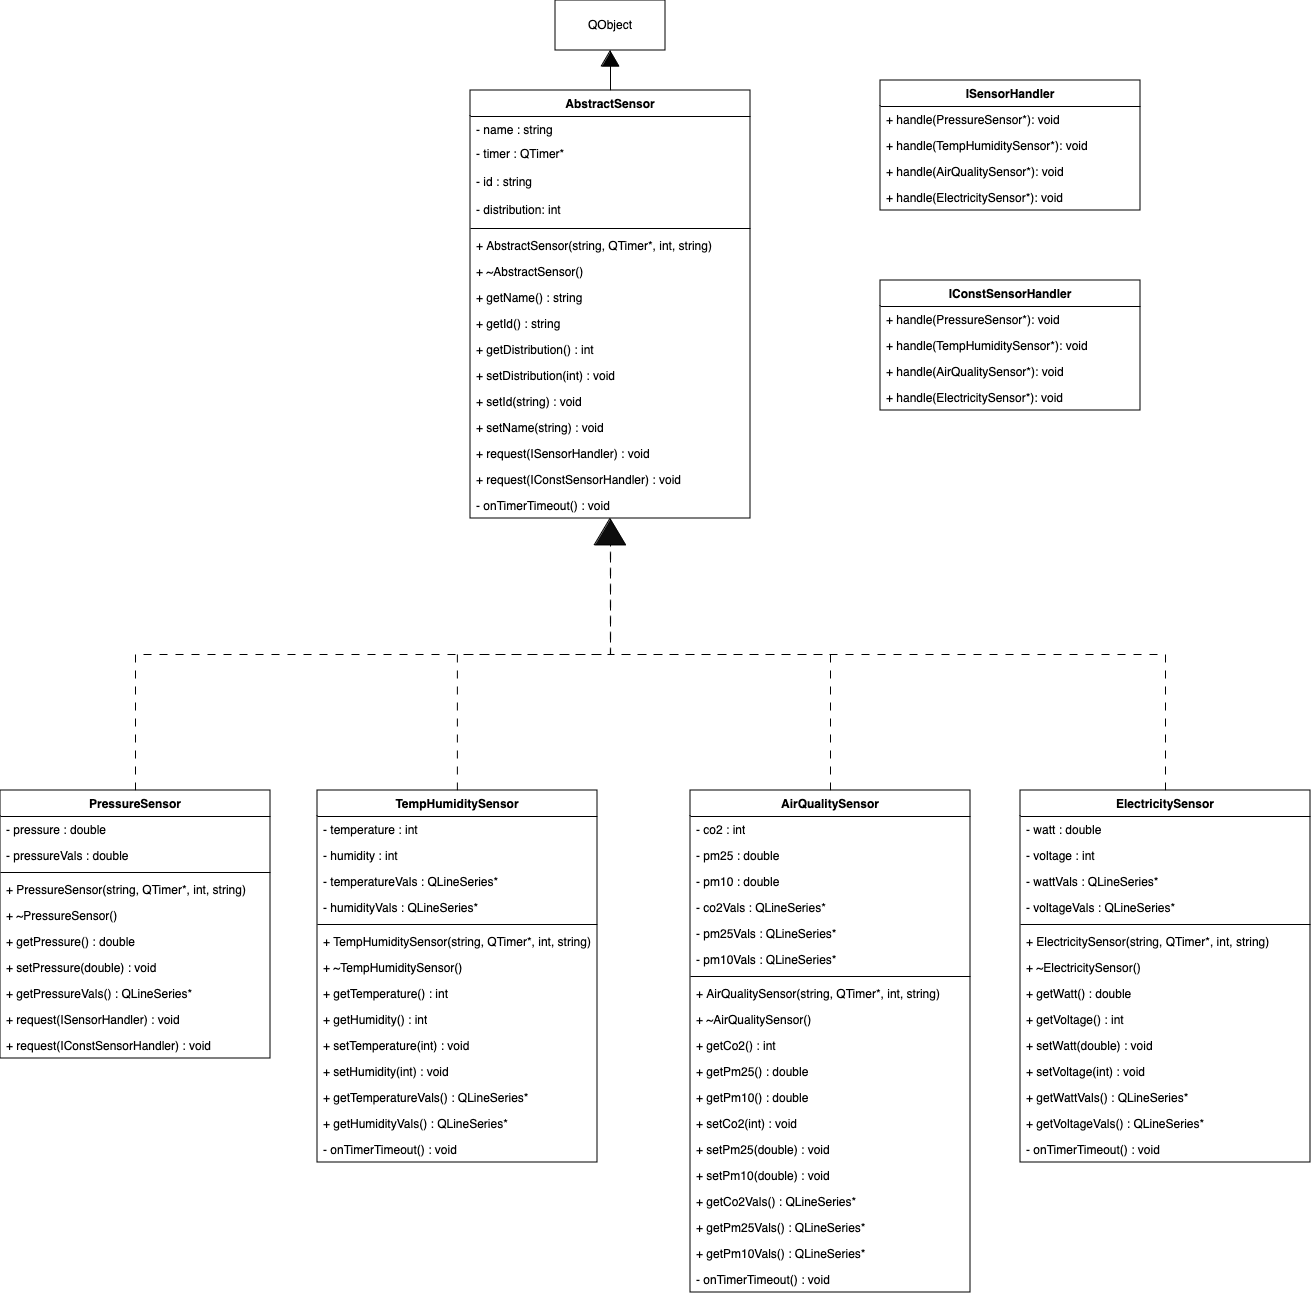
\includegraphics[scale=0.28]{assets/UML.png}
        \caption{Diagramma delle classi dei sensori}
    \end{figure}
    Il modello logico è strutturato in due parti: la prima parte comprende le classi che descrivono i vari sensori utilizzabili all'interno dell'applicativo, mentre la seconda parte si occupa di creazione, lettura e aggiornamento del file JSON che si occupa del salvataggio dei sensori.
    \texttt{AbstractSensor} è la classe base astratta che rappresenta le informazioni comuni a tutti i sensori che possono essere creati, ovvero il nome, il timer, l'identificatore univoco UUID e la tipologia di distribuzione. Oltre ai relativi metodi \emph{getter} e \emph{setter} per le varie variabili d'istanza, 
    è presente il metodo \texttt{onTimerTimeout}, che si occupa di effettuare delle azioni ad ogni \emph{timeout} emesso dal timer: solitamente, le azioni che vengono performate sono quelle di aggiornamento dei valori dei dati che vengono generati dal sensore, oltre a cancellare valori dalle eventuali serie che risultano non necessarie ai fini del funzionamento del software e, in particolare, per la generazione del grafico. Le classi figlie di \texttt{AbstractSensor} sono:
    \begin{itemize}
        \item \texttt{PressureSensor}: descrive il sensore della pressione atmosferica. In particolare, ne indica il valore istantaneo della pressione stessa e gli ultimi venti valori necessari alla generazione del grafico tramite una \texttt{QLineSeries};
        \item \texttt{TempHumidity}: descrive il sensore della temperatura e dell'umidità tramite i valori degli stessi e gli ultimi venti valori necessari alla generazione dei relativi grafici (sempre tramite una \texttt{QLineSeries});
        \item \texttt{AirQualitySensor}: descrive il sensore della qualità dell'aria. I parametri che vengono monitorati e di cui vengono riportati i relativi venti valori per la generazione del grafico sono:
        \begin{itemize}
            \item CO$_2$
            \item PM2.5
            \item PM10
        \end{itemize}
        \item \texttt{ElectricitySensor}: descrive il sensore dell'elettricità, che monitora il consumo istantaneo di energia in Watt e il voltaggio della rete elettrica. Anche per questi ultimi, sono presenti gli ultimi venti valori contenuti all'interno di una \texttt{QLineSeries}
    \end{itemize}
    \section{Polimorfismo}
    L'utilizzo principale del polimorfismo riguarda il \emph{design pattern} \texttt{Visitor} nella gerarchia \texttt{AbstractSensor}. Esso viene utilizzato per:
    \begin{itemize}
        \item per recuperare le \texttt{QLineSeries} dai singoli sensori, necessari per la generazione dei vari grafici relativi ai sensori
        \item per riconoscere la tipologia di sensore
    \end{itemize}
    Le classi che permettono l'esecuzione delle funzionalità sopra elencate sono:
    \begin{itemize}
        \item \texttt{JSONhandler}: per il salvataggio dei sensori viene utilizzato un vector di\\ \texttt{AbstractSensor}, da cui bisognerà ricavare il tipo di sensore che andrà salvato all'interno del JSON;
        \item \texttt{DataPanel}: la seguente classe riceve in input un \texttt{AbstractSensor}; a seconda della tipologia di sensore, l'applicativo dovrà generare un certo numero di grafici di un determinato tipo. 
        Risulta quindi necessario il polimorfismo per modellare la generazione dei grafici a seconda della tipologia di sensore;
        \item \texttt{ItemCard}: la seguente classe si occupa della generazione delle varie card che rappresentano i singoli sensori. Ogni card è caratterizzata
        dal nome del sensore, dai bottoni di eliminazione e modifica, ma soprattutto dalla tipologia di sensore che rappresenta la card. Per ottenere questa informazione, risulta necessario l'utilizzo del polimorfismo.
    \end{itemize}
    Le classi sopra elencate, in quanto effettuano soltanto operazioni di lettura e non di modifica, implementano tutte un \texttt{IConstSensorHandler}, che svolge le funzioni sopra indicate a seconda del tipo concreto del sensore (partendo quindi da un \texttt{AbstractSensor}).
    \section{Persistenza dei dati}
    È necessario avere dei dati persistenti per quanto riguarda tutti i sensori che un utente vuole utilizzare e gestire.
    Per la persistenza dei dati dei sensori viene quindi utilizzato il formato JSON, caratterizzato da un oggetto contente un array di oggetti \texttt{sensors}. 
    Ogni oggetto presente all'interno dell'array \texttt{sensors} rappresenta i dati fondamentali di un singolo sensore:
    \begin{itemize}
    \item \textbf{id}: identificativo univoco del sensore
    \item \textbf{name}: nome del sensore
    \item \textbf{type}: tipologia del sensore
    \item \textbf{distribution}: tipologia di distribuzione dei dati del sensore
    \end{itemize}
    Si riporta un esempio di file JSON \texttt{test.json} nella cartella radice del progetto, contenente un sensore di ogni tipo e di ogni tipologia di distribuzione dei dati 
    per illustrare velocemente il funzionamento del programma.
    \section{Funzionalità implementate}
    Le funzionalità implementate all'interno del programma sono:
    \begin{itemize}
        \item Funzionali
        \begin{itemize}
            \item creazione, gestione e modifica di quattro tipologie di sensori
            \item quattro tipologie di distribuzione dei dati
            \item funzionalità di ricerca mediante RegEx
            \item salvataggio dei sensori in formato JSON
            \item shortcut da tastiera
            \begin{itemize}
                \item CTRL+N per creare un nuovo file JSON
                \item CTRL+O per aprire un file JSON
                \item CTRL+S per salvare le modifiche nel file JSON
                \item CTRL+T per creare un nuovo sensore
                \item CTRL+SHIFT+Backspace per eliminare un sensore che ha il focus
            \end{itemize}
        \end{itemize}
        \item Estetiche
        \begin{itemize}
            \item barra dei menù superiore per gestire le funzionalità relative al file JSON e per eliminare o aggiungere un sensore
            \begin{figure}[H]
                \centering
                
\includegraphics[scale=0.7]{assets/Menu.png}
                \caption{MenuBar in MacOS}
            \end{figure}
            \begin{figure}[H]
                \centering
                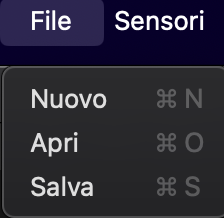
\includegraphics[scale=0.7]{assets/File.png}
                \caption{Menu di gestione del file JSON}
            \end{figure}
            \begin{figure}[H]
                \centering
                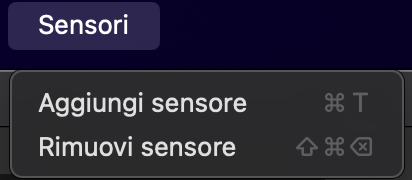
\includegraphics[scale=0.7]{assets/Sensori.png}
                \caption{Menu di gestione del sensore}
            \end{figure}
            \item Presenza di frecce direzionali per cambiare grafico nel caso in cui fossero più di uno
            \begin{figure}[H]
                \centering
                
\includegraphics[scale=0.6]{assets/Buttons.png}
                \caption{Freccie direzionali}
            \end{figure}
            \item bottoni clickabili per ogni sensore per effettuare modifica o eliminazione sul singolo
            \begin{figure}[H]
                \centering
                
\includegraphics[scale=0.7]{assets/ButtonSensori.png}
                \caption{Item Card}
            \end{figure}
            \item cambio del colore del bordo tramite hover del mouse
            \begin{figure}[H]
                \centering
                
\includegraphics[scale=0.7]{assets/ItemCard.png}
                \caption{Item Card}
            \end{figure}
        \end{itemize}
    \end{itemize}
    \section{Rendicontazione ore}
    \begin{center}
        \begin{tabular}{|l|c|c|}
            \hline
            \textbf{Attività} & \textbf{Ore Previste} & \textbf{Ore effettive} \\
            \hline
            Studio e progettazione grafica & 5 & 6 \\
            \hline
            Studio del framework Qt & 15 & 18 \\
            \hline
            Sviluppo del codice del modello & 8 & 9 \\
            \hline
            Sviluppo del codice della GUI & 20 & 22 \\
            \hline
            Test e debug & 5 & 8 \\
            \hline
            Stesura della relazione & 5 & 5 \\
            \hline
            \textbf{Totale} & 58 & \textbf{68} \\
            \hline
        \end{tabular}
    \end{center}
    Il monte ore è stato superato di 10 ore circa a causa di una serie di problemi; una delle attività che ha subito più ritardo nella tabella di marcia è stato sicuramente lo studio del framework Qt in quanto sottostimato come tempo e consuntivato prendendo spunto dalle stime orarie fornite dal professore. L'attività, ovviamente, comprende anche delle ore di sviluppo codice del software, utilizzato per prendere confidenza con il framework e ridurre il tempo sprecato.
    Un altro evento che ha richiesto più tempo del dovuto è stato sicuramente la fase di Test e debug; i principali problemi riscontrati durante lo sviluppo che hanno richiesto molto tempo per il debug sono:
    \begin{itemize}
        \item \textbf{conflitti di focus}: il programma crashava a seguito della perdita di focus del sensore, che causava l'eliminazione del data panel (come da progetto), che però aveva appena acquisito il focus;
        \item \textbf{perdita di focus dovuta ai popup menu}: data la poca esperienza con il framework, uno dei problemi che ha richiesto del tempo nella fase di test e debug è quella dei popup menu del QMenu all'interno della QMenuBar. Questi, nonostante la focus policy fosse impostata a \texttt{Qt::NoFocus}, il popup menu acquisiva comunque il focus, non permettendo così l'eliminazione tramite menù.
    \end{itemize}
\end{document}